\begin{frame}
  \begin{center}
    \Huge Properties
  \end{center}
\end{frame}

\begin{frame}
  \frametitle{Properties}
  \framesubtitle{Node state/label I}
  Let
  \begin{itemize}
    \item \blue{$P_i$} be an elementary path from \blue{$s$} to \blue{$i \in V$} in \blue{$D$}; and 
    \item \blue{$S_i = (L_i = (l^1_i, ..., l^{|R|}_i), C_i)$} be the state or label of node \blue{$i \in V(P_i)$} in the path \blue{$P_i$}, where:
    \begin{itemize}
      \item \blue{$l^r_i \in \mathbb{R}_{+}$} is the amount of resource \blue{$r \in R$} consumed by the path \blue{$P_i$} at \blue{$i \in V(P_i)$}; and 
      \item \blue{$C_i \in \mathbb{R}$} is the cost of path \blue{$P_i$} at \blue{$i \in V(P_i)$}.
    \end{itemize}
  \end{itemize}
\end{frame}

\begin{frame}
  \frametitle{Properties}
  \framesubtitle{Node state/label I}
  \blue{$P_2, S_3 = (L_3 = (2, 2), 1), S_2 = (L_2 = (3, 0), 5)$}
  \begin{figure}[H]
    \centering
    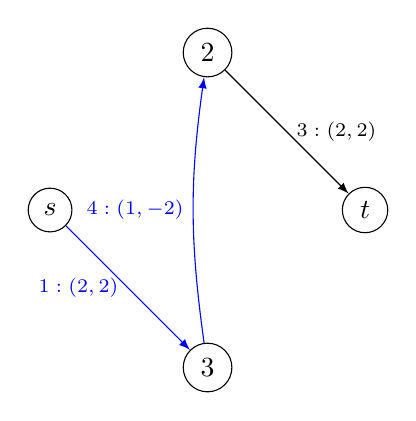
\begin{tikzpicture}
      %nodes
      \node[circle, draw] (s) at (0, 0) {\blue{$s$}};
      \node[circle, draw] (a) at (2, 2) {\blue{$2$}};
      \node[circle, draw] (b) at (2, -2) {\blue{$3$}};
      \node[circle, draw] (t) at (4, 0) {\blue{$t$}};
      %edges
      \path [blue, draw,-latex] (s) to node[left]{\scriptsize\blue{$1: (2, 2)$}} (b);
      \path [blue, draw,-latex] (b) edge [bend left=8] node[left]{\scriptsize\blue{$4: (1, -2)$}} (a);
      \path [draw,-latex] (a) to node[right]{\scriptsize\blue{$3: (2, 2)$}} (t);
    \end{tikzpicture}
    \caption{\blue{$P_2$}.}
    \label{fig:vrptw_disposable_example}
  \end{figure}
\end{frame}

\begin{frame}
  \frametitle{Properties}
  \framesubtitle{Dominance I}
  Let
  \begin{itemize}
    \item \blue{$P_i$} and \blue{$P^{'}_i$} be two distinct elementary paths from \blue{$s$} to \blue{$i \in V$} in \blue{$D$}; and
    \item \blue{$S_i$} and \blue{$S^{'}_i$} be the respective labels.
  \end{itemize}
  \begin{definition}
    \blue{$P_i$} dominates \blue{$P^{'}_i \leftrightarrow S_i \leqslant S^{'}_i$}.
  \end{definition}
\end{frame}

\begin{frame}
  \frametitle{Properties}
  \framesubtitle{Node state/label II}
  Let
  \begin{itemize}
    \item \blue{$L_i = (l^1_i, ..., l^{|R|}_i, s_i, v_i^1, ..., v_i^{|V|})$} be the the  new resources state/label, where:
      \item the number of visited nodes, and the visitation vector by the path \blue{$P_i$}.
    \begin{itemize}
      \item \blue{$l^r_i \in \mathbb{R}_{+}$} is the amount of resource \blue{$r \in R$} consumed by the path \blue{$P_i$} at \blue{$i \in V(P_i)$};
      \item \blue{$s_i = \sum_{j = 1}^{|V|} v_i^j$} is the number of nodes visited by the path \blue{$P_i$} at \blue{$i \in V(P_i)$}; and 
      \item \blue{$v_i^j \in \mathbb{B}$} is equals to \blue{$1$} if node \blue{$j \in V$} is visited by the path \blue{$P_i$} at \blue{$i \in V(P_i)$} and \blue{$0$} otherwise.
    \end{itemize}
  \end{itemize}
\end{frame}

\begin{frame}
  \frametitle{Properties}
  \framesubtitle{Node state/label II}
  \blue{$P_2, S_s = (L_s = (0, 0, 1, 1, 0, 0, 0), 0) , S_3 = (L_3 = (2, 2, 2, 1, 0, 1, 0), 1), S_2 = (L_2 = (3, 0, 3, 1, 1, 1, 0), 5)$}
  \begin{figure}[H]
    \centering
    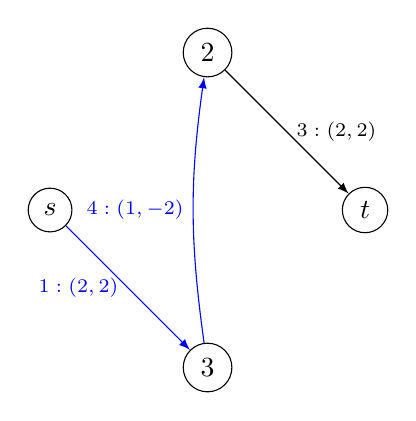
\begin{tikzpicture}
      %nodes
      \node[circle, draw] (s) at (0, 0) {\blue{$s$}};
      \node[circle, draw] (a) at (2, 2) {\blue{$2$}};
      \node[circle, draw] (b) at (2, -2) {\blue{$3$}};
      \node[circle, draw] (t) at (4, 0) {\blue{$t$}};
      %edges
      \path [blue, draw,-latex] (s) to node[left]{\scriptsize\blue{$1: (2, 2)$}} (b);
      \path [blue, draw,-latex] (b) edge [bend left=8] node[left]{\scriptsize\blue{$4: (1, -2)$}} (a);
      \path [draw,-latex] (a) to node[right]{\scriptsize\blue{$3: (2, 2)$}} (t);
    \end{tikzpicture}
    \caption{\blue{$P_2$}.}
    \label{fig:vrptw_disposable_example}
  \end{figure}
\end{frame}

\begin{frame}
  \frametitle{Properties}
  \framesubtitle{Dominance II}
  Let
  \begin{itemize}
    \item \blue{$P_i$} and \blue{$P^{'}_i$} be two distinct elementary paths from \blue{$s$} to \blue{$i \in V$} in \blue{$D$}; and
    \item \blue{$S_i$} and \blue{$S^{'}_i$} be the paths respective labels.
  \end{itemize}
  \begin{definition}
    \blue{$P_i$} dominates \blue{$P^{'}_i \leftrightarrow S_i \leqslant S^{'}_i$}.
  \end{definition}
\end{frame}

\begin{frame}
  \frametitle{Properties}
  \framesubtitle{Unreachable nodes}
  Let
  \begin{itemize}
    \item \blue{$P_i$} be an elementary path from \blue{$s$} to \blue{$i \in V$} in \blue{$D$}; 
    \item \blue{$S_i$} be the path label; and
    \item \blue{$k \in V$} be a digraph node.
  \end{itemize}
  \begin{definition}
    \blue{$k$} is said to be unreachable by \blue{$P_i \rightarrow k \in V(P_i) \vee \exists r \in R (l_i^r + d_{ik}^r > e^r_k)$}.
  \end{definition}
  Note that, does not exist any path from \blue{$i$} that permits to reach it, due to the digraph metricity.
\end{frame}

\begin{frame}
  \frametitle{Properties}
  \framesubtitle{Node state/label III}
  Let
  \begin{itemize}
    \item \blue{$L_i = (l^1_i, ..., l^{|R|}_i, s_i, v_i^1, ..., v_i^{|V|})$} be the the new resources state/label, where:
      \item the number of visited nodes, and the visitation vector by the path \blue{$P_i$}.
    \begin{itemize}
      \item \blue{$l^r_i \in \mathbb{R}_{+}$} is the amount of resource \blue{$r \in R$} consumed by the path \blue{$P_i$} at \blue{$i \in V(P_i)$};
      \item \blue{$s_i = \sum_{j = 1}^{|V|} v_i^j$} is the number of unreachable nodes by the path \blue{$P_i$} at \blue{$i \in V(P_i)$}; and 
      \item \blue{$v_i^j \in \mathbb{B}$} is equals to \blue{$1$} if node \blue{$j \in V$} is unreachable by the path \blue{$P_i$} at \blue{$i \in V(P_i)$} and \blue{$0$} otherwise.
    \end{itemize}
  \end{itemize}
\end{frame}

\begin{frame}
  \frametitle{Properties}
  \framesubtitle{Nondominated paths}
  \begin{claim}
    In order to find the ERCSPP optimal solution, suffices to consider only nondominated paths.
  \end{claim}
  \begin{claimproof}
    Let's consider two elementary paths \blue{$P_i$} and \blue{$P^{'}_i$} from \blue{$s$} to \blue{$i \in V$}, along with its labels \blue{$S_i$} and \blue{$S^{'}_i$}, such that \blue{$P_i$} dominates \blue{$P^{'}_i$}.
    Also, let's consider an arc \blue{$(i, j) \in A : \forall r \in R (l_i^{'r} + d_{ij}^r \leqslant e_j^r) \wedge v_i^{'j} = 0$}.
    Note that \blue{$\forall r \in R (l_i^r + d_{ij}^r \leqslant e_j^r) \wedge v_i^{j} = 0 \wedge C_i \leqslant C^{'}_i$}.
  \end{claimproof}
\end{frame}
